%\begin{frame}{Opgave 3: Adaptiv kvadraturregler}
%    Forklar idéen i en sammensat adaptiv kvadraturregel.
%\end{frame}

\begin{frame}{Adaptiv kvadraturregler}
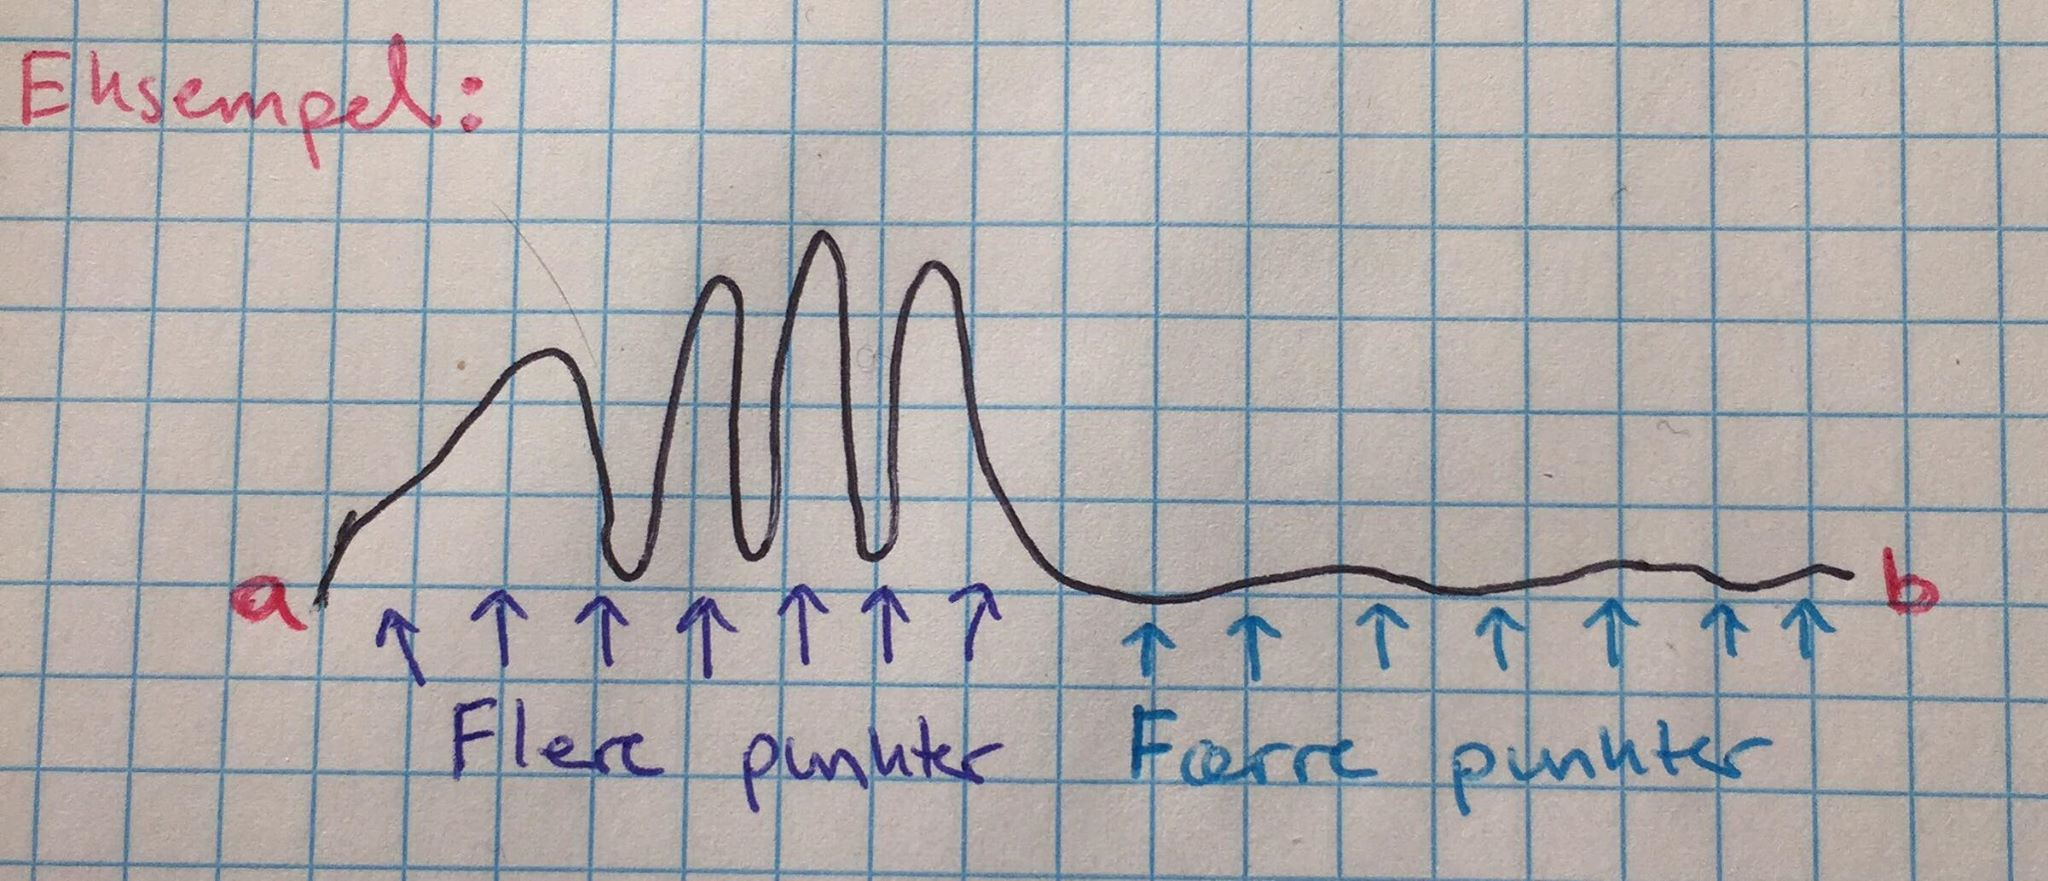
\includegraphics[scale=0.15]{images/Adaptiv_eks.png}
%
%
\end{frame}
\begin{frame}{Adaptiv kvadratur}
\phantom{H} \\
\centering
%
%%%%%%%%%%%%%%%%%%%%%%%%%%%%%%%%
%%% Flot graf alla Julie     %%%
%%%%%%%%%%%%%%%%%%%%%%%%%%%%%%%%
%
{\small
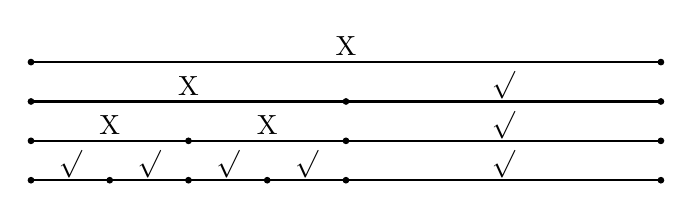
\begin{tikzpicture}[scale=1]
%
\draw[thick] (0,0) -- (8,0);
\filldraw [black] (0,0) circle (1pt);
\filldraw [black] (1,0) circle (1pt);
\filldraw [black] (2,0) circle (1pt);
\filldraw [black] (3,0) circle (1pt); 
\filldraw [black] (4,0) circle (1pt);
\filldraw [black] (8,0) circle (1pt); 
\node at (0.5,0.2) (){$\mathcal{p}$};
\node at (1.5,0.2) (){$\mathcal{p}$};
\node at (2.5,0.2) (){$\mathcal{p}$};
\node at (3.5,0.2) (){$\mathcal{p}$};
\node at (6,0.2) (){$\mathcal{p}$}; 
%
\draw[thick] (0,0.5) -- (8,0.5);
\filldraw [black] (0,0.5) circle (1pt);
\filldraw [black] (2,0.5) circle (1pt); 
\filldraw [black] (4,0.5) circle (1pt); 
\filldraw [black] (8,0.5) circle (1pt); 
\node at (1,0.7) (){X};
\node at (3,0.7) (){X};
\node at (6,0.7) (){$\mathcal{p}$}; 
%
\draw[thick] (0,1) -- (8,1);
\filldraw [black] (0,1) circle (1pt); 
\filldraw [black] (4,1) circle (1pt); 
\filldraw [black] (8,1) circle (1pt);
\node at (2,1.2) (){X};
\node at (6,1.2) (){$\mathcal{p}$};
%
\draw[thick] (0,1.5) -- (8,1.5);
\filldraw [black] (0,1.5) circle (1pt); 
\filldraw [black] (8,1.5) circle (1pt); 
\node at (4,1.7) (){X};
%
\end{tikzpicture}
}
\end{frame}